\chapter{进程}

    \emph{进程是任何躲到程序涉及的操作系统中的基本概念}

\section{进程、轻量级进程和线程}

    OS教科书的常规定义:\emph{进程是程序执行时的一个实例。}每一个进程都只有一个父亲。

    从内核的观点来看:\emph{进程的目的就是担当分配系统资源(CPU time、memory)的实体。}

    对于一个进程的创建,其原理是接受父进程地址空间的一个(逻辑)拷贝。\emph{尽管父子进程可以共享含有程序代码(正文)的页,但是拥有各自独立的数据拷贝,因此子进程对内存单元的修改对父进程是不可见的(反之亦然)}

    对于现代Unix系统来说,需要支持多线程应用————\emph{拥有很多相对独立执行流的用户程序共享应用的大部分数据结构。}这样的系统中,进程由多个线程组成,每个线程都代表进程的一个执行流。

    目前而言,大多数多线程应用都是基于pthread(POSIX thread)库的标准库函数集编写的

    Linux使用轻量级进程(lightweight process)对多线程进行更好的支持。\emph{对于轻量级进程而言,可以共享资源,只要其中一个修改共享资源,另一个就会立即查看并同步。}

\subsection{进程描述符}

    进程描述符(process descriptor,由task\_struct类修饰),其字段包含了与进程相关的所有信息。

\begin{figure}[!htbp]
    \centering
    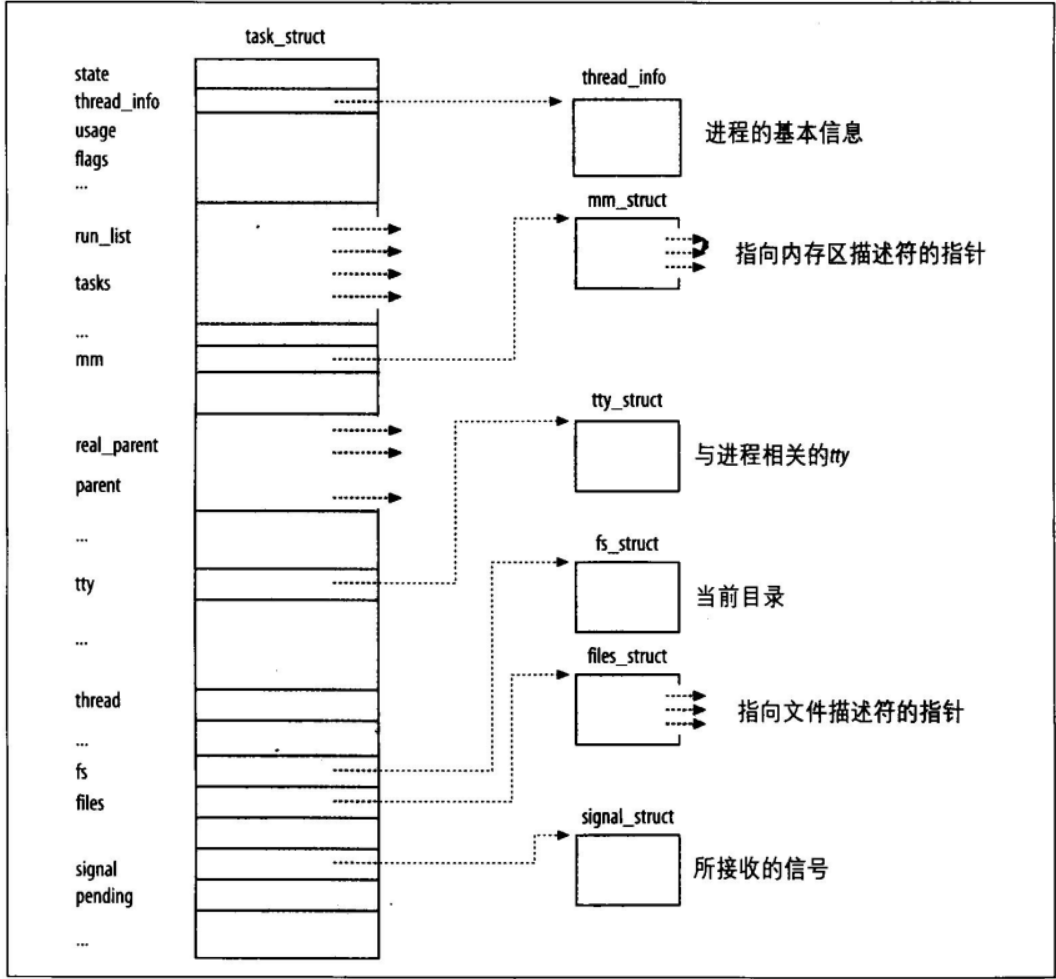
\includegraphics[width=0.8\textwidth]{image/chapter03/Linux进程描述符.png}
    \caption{Linux进程描述符}
\end{figure}

    图3-1右边的六个数据结构涉及进程拥有的所有特殊资源,目前我们只讨论两种:进程的状态以及进程的父子关系

\subsection{进程状态}

    进程描述符中的state字段描述了当前进程所处的状态。其由一组标志组成,其中每一个标志描述了一种可能的进程状态。

    值得注意的是:\emph{状态之间是互斥的,严格意义上只允许存在一种状态。}

\begin{lstlisting}[language=C++, caption={进程状态一览}]
#define TASK_RUNNING		    0
#define TASK_INTERRUPTIBLE	    1
#define TASK_UNINTERRUPTIBLE	2
#define TASK_STOPPED		    4
#define TASK_TRACED		        8
#define EXIT_ZOMBIE		        16
#define EXIT_DEAD		        32
\end{lstlisting}

\begin{itemize}
    \item TASK\_RUNNING
    \subitem 进程要么已经执行,要么准备执行
    \item TASK\_INTERRUPTIBLE
    \subitem 进程被挂起,知道某个条件为真。产生硬件中断,释放进程正在等待的系统资源或传递一个信号都是可以唤醒进程的条件(也就是恢复到TASK\_RUNNING)
    \item TASK\_UNINTERRUPTIBLE
    \subitem 与上一个状态类似,但传递信号无法唤醒。\emph{一般用于特殊情况下,进程必须等待,直到一个不能被中断的实践发生}
    \item TASK\_STOPPED
    \subitem 进程的执行被暂停,当接收到SIGSTOP、SIGTSTP、SIGTTIN和SIGTTOU信号后,进入暂停
    \item TASK\_TRACED
    \subitem 进程的执行由debugger程序暂停。当一个进程被另一个进程监控时,任何信号都可以把这个进程置于TASK\_TRACED状态
    \item EXIT\_ZOMBIE
    \subitem 进程的执行被终止,但是父进程未发布wait()类系统调用来返回有关死亡进程的信息
    \item EXIT\_DEAD
    \subitem 最终状态,由于父进程刚发布wait()类系统调用,因而进程被系统删除,但防止其他线程也执行wait()类系统调用,为了防止冲突,因而将僵死状态设置为僵死撤销(将亡)状态
\end{itemize}

    一般的,进程状态可以由以下简单的赋值语句设置,也可以由宏设置:

\begin{lstlisting}[language=C++]
p->state = TASK_RUNNING;

#define __set_task_state(tsk, state_value)		\
	do { (tsk)->state = (state_value); } while (0)
#define set_task_state(tsk, state_value)		\
	set_mb((tsk)->state, (state_value))

#define __set_current_state(state_value)			\
	do { current->state = (state_value); } while (0)
#define set_current_state(state_value)		\
	set_mb(current->state, (state_value))
\end{lstlisting}

\subsection{标识一个进程}

    进程和进程描述符之间有非常严格的一一对应关系,这使得进程描述符标识进程称为一种方便的方式。

    另一方面,类Unix操作系统允许用户使用进程标识符process ID(PID)来标识进程,PID存放在进程描述符的pid字段中。

    PID被顺序编号,新创建的进程通常是前一个PID加1。PID的值通常有一个上线,缺省情况下,最大PID号是32767(PID\_MAX\_DEFAULT - 1)

    由于循环使用PID,因此需要通过与个pidmap\_array位图来标识当前已分配的PID和闲置的PID。

    Linux希望同一个线程组内有同一个PID,因此,\emph{一个线程组中的所有线程使用和该线程组的领头线程的PID,被存放在进程描述符中的tgid字段。}系统调用getpid()实际上是返回的tgid的值,而非PID。

\subsection{进程描述符处理}

    进程是动态实体,因此内核必须能够同时处理多进程,并把进程描述符存放在动态内存中,而非在永久分配给内核的内存区。

    对于每个进程来说,Linux把内核态的进程堆栈和进程描述符中的thread\_info(线程描述符)紧凑的存放在一个单独的存储区域内。

\begin{figure}[!htbp]
    \centering
    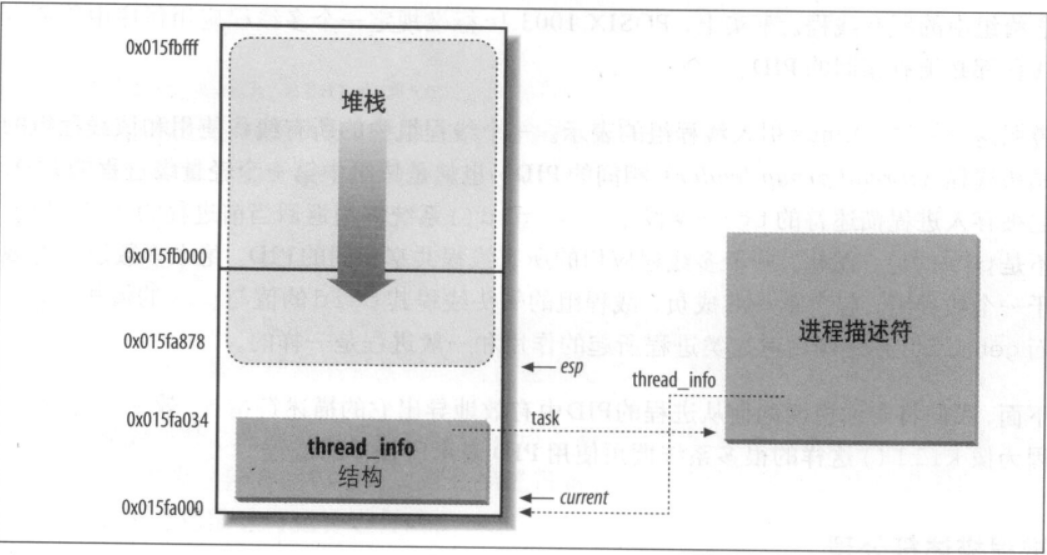
\includegraphics[width=0.8\textwidth]{image/chapter03/thread_info与进程内核栈.png}
    \caption{thread\_info结构和进程内核栈存放在两个连续的页框中}
\end{figure}

    线程描述符驻留于该内存区的开始,栈从末端向下开始增长。

    esp寄存器是CPU的栈指针(x86架构),用来存放栈顶单元的地址。栈起始于末端,并朝该内存区开始的地方开始增长。\emph{从用户态切换到内核态后,进程的内核总是空的}

    在内核中,使用union对该结构进行描述:

\begin{lstlisting}[language=C++]
#define THREAD_SIZE     (4096)
#else
#define THREAD_SIZE		(8192)
#endif

union thread_union {
    struct thread_info thread_info;
    unsigned long stack[THREAD_SIZE/sizeof(long)];
};
\end{lstlisting}

\subsection{标识当前进程}

    从效率上看:\emph{thread\_info结构体与内核态堆栈之间的紧密结合提供的主要好处为:内核可以轻易从esp的值获取CPU正在运行进程的thread\_info的地址}

    事实上,如果thread\_union结构长度是8K($2^{13}$),则内核屏蔽掉esp的低13位有效位就能够获取thread\_info的基地址。这项工作由以下函数实现:

\begin{lstlisting}[language=C++]
/* how to get the thread information struct from C */
static inline struct thread_info *current_thread_info(void)
{
    struct thread_info *ti;
    __asm__("andl %%esp,%0; ":"=r" (ti) : "0" (~(THREAD_SIZE - 1)));
    return ti;
}
\end{lstlisting}

    也就是说,通过该函数内联汇编:

\begin{lstlisting}[language=C++]
movl $0xffffe000, %ecx
andl %esp, %ecx
movl %ecx, p
\end{lstlisting}

    这样执行后,p就包含了CPU当前运行进程的thread\_info结构的指针。

    但是,进程中最常用的是进程描述符的地址而非thread\_info的地址,因此,内核需要调用current宏,其等价于

\begin{lstlisting}[language=C++]
current_thread_info()->task;

movl $0xffffe000, %ecx
andl %esp, %ecx
movl (%ecx), p
\end{lstlisting}

    查看源码可以知道,task在thread\_info上的偏移量是0,因此上述三条指令就能够将进程描述符指针赋值到p上。

\subsection{双向链表}

    对于每一个链表,都需要实现一组原语操作:初始化,插入和删除,遍历等操作。Linux内核定义了list\_head数据结构,字段next和prev分别表示通用黄翔链表向前和向后的指针元素。

\begin{lstlisting}[language=C++]
struct list_head {
    struct list_head *next, *prev;
};
\end{lstlisting}

\begin{figure}[!htbp]
    \centering
    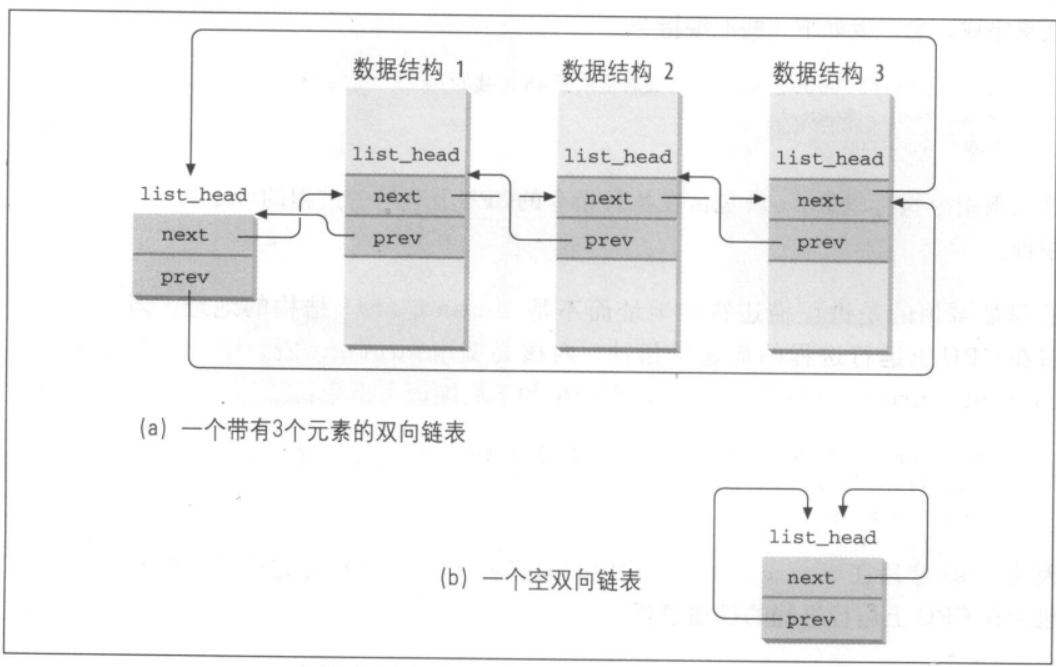
\includegraphics[width=0.6\textwidth]{image/chapter03/list_head构造双向链表.png}
    \caption{list\_head构造双向链表}
\end{figure}

    对于新链表而言,是用LIST\_HEAD(list\_name)宏创建的,其声明类型为list\_head的新变量list\_name。见上图中b图。Linux内核为链表提供了一些原语操作:

\begin{lstlisting}[language=C++]
// 初始化链表
#define LIST_HEAD_INIT(name) { &(name), &(name) }
#define LIST_HEAD(name) \
    struct list_head name = LIST_HEAD_INIT(name)
// 链表头插
static inline void list_add(
    struct list_head *new, struct list_head *head)
{
    __list_add(new, head, head->next);
}
// 链表尾插
static inline void list_add_tail(
    struct list_head *new, struct list_head *head)
{
	__list_add(new, head->prev, head);
}
// 链表删除
static inline void list_del(struct list_head *entry)
{
	__list_del(entry->prev, entry->next);
	entry->next = LIST_POISON1;
	entry->prev = LIST_POISON2;
}
// 链表判空
static inline int list_empty(const struct list_head *head)
{
	return head->next == head;
}
// 获取链表元素
#define list_entry(ptr, type, member) \
	container_of(ptr, type, member)
// 遍历链表
#define list_for_each(pos, head) \
for (pos = (head)->next; prefetch(pos->next), pos != (head); \
        pos = pos->next)

#define list_for_each_entry(pos, head, member)				\
for (pos = list_entry((head)->next, typeof(*pos), member);	\
        prefetch(pos->member.next), &pos->member != (head); 	\
        pos = list_entry(pos->member.next, typeof(*pos), member))
\end{lstlisting}

\subsubsection{进程链表}

    进程链表把所有的进程描述符链接起来。每一个task\_struct结构都包含一个list\_head类型的tasks字段,prev和next分贝指向前后的task\_struct元素。

    进程链表的头是init\_struct描述符,也就是0进程(process 0)或swapper进程的进程描述符。

    SET\_LINKS和REMOVE\_LINKS分别用于从进程链表中插入和删除一个进程描述符,且考虑了父子进程间关系。同时也有宏for\_each\_process,遍历整个进程链表。

\begin{lstlisting}[language=C++]
#define next_task(p)	\
    list_entry((p)->tasks.next, struct task_struct, tasks)
#define prev_task(p)	\
    list_entry((p)->tasks.prev, struct task_struct, tasks)
#define for_each_process(p) \
    for (p = &init_task ; (p = next_task(p)) != &init_task ; )
\end{lstlisting}

\subsubsection{TASK\_RUNNING状态的进程链表}

    当内核寻找新进程运行时,\emph{只需要考虑处于TASK\_RUNNING状态的进程}

    早先的Linux把可运行进程都放在运行队列(runqueue)的链表中,但是维持链表中进程优先级排序的开销过大,因此早期的调度程序不得不为选择最佳可运行程序而扫描整个进程。

    而2.6实现的运行队列,目的是为了\emph{让调度程序在固定时间内选出最佳可运行进程,与队列中可运行的进程数无关。}

    \emph{提高调度程序运行速度的诀窍是建立多个可运行进程链表,每种进程优先级对应一个不同的链表。}

    每个task\_struct描述符包含一个list\_head类型的字段run\_list,如果进程优先级等于k(取值为0~139),run\_list就把该进程链入优先级为k的可运行进程队列中。

    在内核中,运行队列的主要数据结构还是组成运行队列的进程描述符链表,所有这些链表都由一个单独prio\_array\_t数据结构来实现

\begin{lstlisting}[language=C++]
struct prio_array {
    // 链表中进程描述符的数量
    unsigned int nr_active;
    // 优先权位图,仅当某个优先权的进程链表不为空时设置
    unsigned long bitmap[BITMAP_SIZE];
    // 140个优先权队列的头节点
    struct list_head queue[MAX_PRIO];
};

typedef struct prio_array prio_array_t;

static void enqueue_task(struct task_struct *p, prio_array_t *array)
{
	sched_info_queued(p);
	list_add_tail(&p->run_list, array->queue + p->prio);
	__set_bit(p->prio, array->bitmap);
	array->nr_active++;
	p->array = array;
}
\end{lstlisting}

    enqueue\_task把进程描述符插入某个运行队列的链表,进程描述符的prio字段存放进程的动态优先权,array时一个指针,指向当前队列的prio\_array\_t数据结构。

\subsection{进程间的关系}

    程序创建的进程具有父/子关系,而一个进程创建多个子进程,子进程之间具有兄弟关系。

    因此,进程描述符中引入几个字段表示这些关系。\emph{进程0和进程1由内核创建}

\begin{lstlisting}[language=C++]
/* real parent process (when being debugged) */
struct task_struct *real_parent; 
struct task_struct *parent;	/* parent process */
/*
* children/sibling forms the list of my children plus the
* tasks I'm ptracing.
*/
/* list of my children */
struct list_head children;	
/* linkage in my parent's children list */
struct list_head sibling;	
\end{lstlisting}

    下图中演示了一组进程间的关系:

\begin{figure}[!htbp]
    \centering
    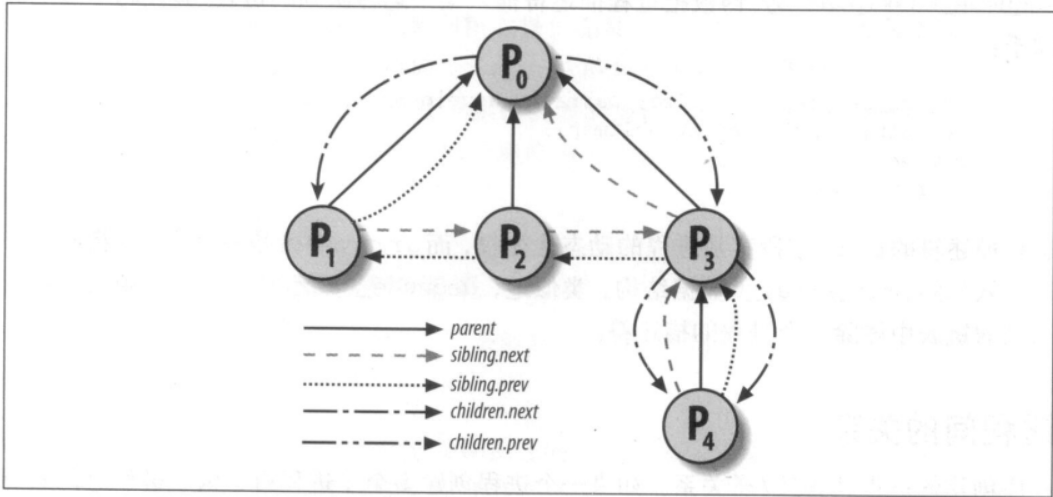
\includegraphics[width=0.8\textwidth]{image/chapter03/五个进程间的亲属关系.png}
    \caption{五个进程间的亲属关系}
\end{figure}

    值得注意的是,\emph{一个进程可能是一个进程组或登录会话的领头进程,也可能是线程组的临潼进程,还可能是跟踪其他进程执行}

\begin{lstlisting}[language=C++]
group_leader        // P所在进程组的领头进程描述符指针
signal->pgrp        // P所在进程组的领头进程PID
tgid                // P所在线程组的领头进程PID
signal->session     // P的登录会话领头进程PID
ptrace_children     // 链表头部,包含所有被debugger程序跟踪子线程
ptrace_list         // 跟踪进程父进程链表的前后元素
\end{lstlisting}

\subsubsection{pidhash表及链表}

    在一些情况下,内核必须从进程的PID导出对应的进程描述符指针:为kill()系统调用提供服务

    顺序扫描进程链表并检查进程描述符PID的做法可行,但是相当低效。为了快速查找,引入了4个散列表。引入4个散列表的原因是:进程描述符包含了表示不同类型的PID字段,每种PID都需要自己的散列表

\begin{table*}[!htbp]
    \begin{center}
        \caption{散列表和进程描述符中的相关字段}
        \begin{tabular}{c c c}
            \hline
            Hash表的类型 & 字段名 & 说明 \\
            PIDTYPE\_PID & pid & 进程的PID \\
            PIDTYPE\_TGID & tgid & 进程组领头进程的PID \\
            PIDTYPE\_PGID & pgrp & 线程组领头进程的PID \\
            PIDTYPE\_SID & session & 会话领头进程的PID \\
            \hline
        \end{tabular}
    \end{center}
\end{table*}

    \emph{内核初始化期间动态地为4个散列表分配空间,并把它们的地址存入pid\_hash数组}

    用pid\_hashfn宏把PID转化为表索引:

\begin{lstlisting}[language=C++]
#if BITS_PER_LONG == 32
/* 2^31 + 2^29 - 2^25 + 2^22 - 2^19 - 2^16 + 1 */
#define GOLDEN_RATIO_PRIME 0x9e370001UL
#elif BITS_PER_LONG == 64
/*  2^63 + 2^61 - 2^57 + 2^54 - 2^51 - 2^18 + 1 */
#define GOLDEN_RATIO_PRIME 0x9e37fffffffc0001UL
#else
#error Define GOLDEN_RATIO_PRIME for your wordsize.
#endif

#define pid_hashfn(nr) hash_long((unsigned long)nr, pidhash_shift)

static inline unsigned long hash_long(unsigned long val, unsigned int bits)
{
	unsigned long hash = val;

#if BITS_PER_LONG == 64
	/*  Sigh, gcc can't optimise this alone like it does for 32 bits. */
	unsigned long n = hash;
	n <<= 18; hash -= n;
	n <<= 33; hash -= n;
	n <<= 3; hash += n;
	n <<= 3; hash -= n;
	n <<= 4; hash += n;
	n <<= 2; hash += n;
#else
	/* On some cpus multiply is faster, on others gcc will do shifts */
	hash *= GOLDEN_RATIO_PRIME;
#endif

	/* High bits are more random, so use them. */
	return hash >> (BITS_PER_LONG - bits);
}
\end{lstlisting}

    但是,我们清楚:\emph{散列(hash)函数并不总能确保PID与表的索引一一对应,两个不同的PID散列到相同的表索引被称为冲突(colliding)}

    Linux利用链表来处理冲突的PID:\emph{每个表项是由冲突的进程描述符组成的双向链表}

\begin{figure}[!htbp]
    \centering
    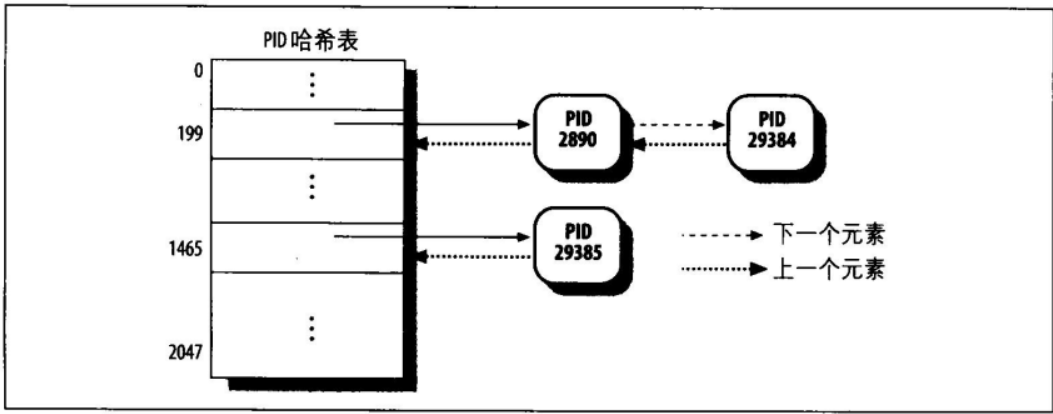
\includegraphics[width=0.8\textwidth]{image/chapter03/pidhash表及链表.png}
    \caption{pidhash表及链表}
\end{figure}

    可以看见,PID2890和PID29384被散列到第200的元素处,然后通过双向链表进行链接。

    \emph{具有链表的散列法比PID到表索引的线性转换更为优越,因为系统中的进程数总是远远小于32768。}

    PID散列表的数据结构解决了上述的难题,最主要的数据结构是四个PID结构的素组,其在进程描述符的PID字段中:

\begin{lstlisting}[language=C++]
enum pid_type
{
	PIDTYPE_PID,
	PIDTYPE_TGID,
	PIDTYPE_PGID,
	PIDTYPE_SID,
	PIDTYPE_MAX
};

struct pid
{
    // pid的数值
	int nr;
    // 链接散列表的前后元素
	struct hlist_node pid_chain;
	// 每一个pid的进程链表头
	struct list_head pid_list;
};
\end{lstlisting}

\begin{figure}[!htbp]
    \centering
    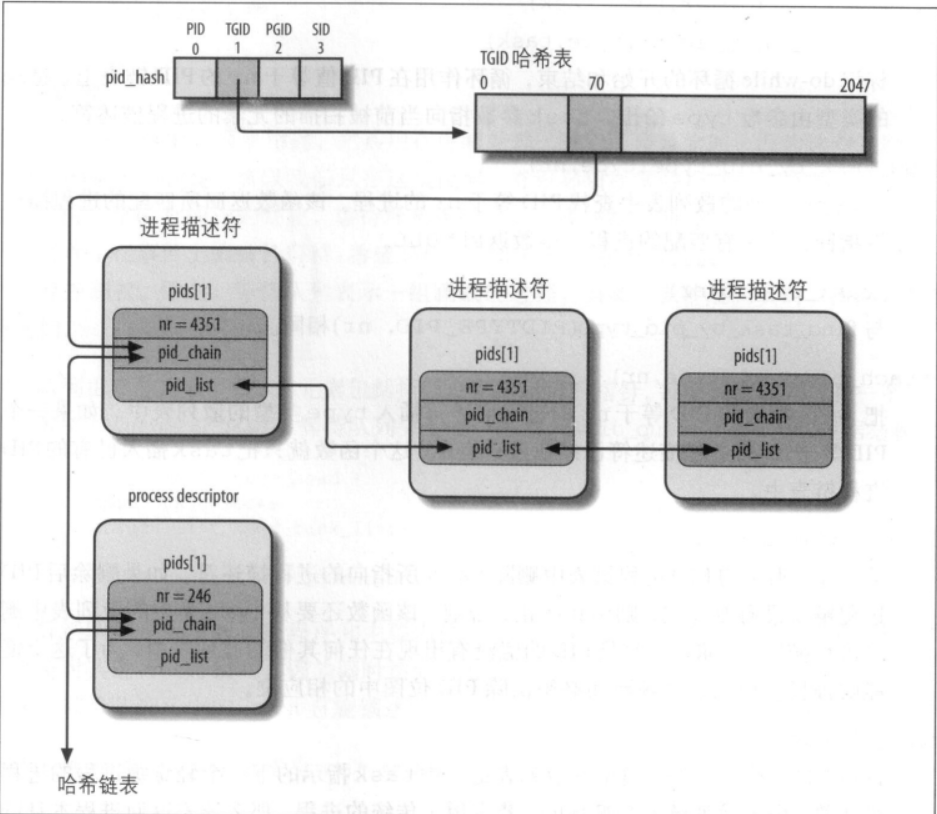
\includegraphics[width=0.8\textwidth]{image/chapter03/pid散列表.png}
    \caption{pid散列表}
\end{figure}

    下面是处理PID散列表的函数和宏:

\begin{itemize}
    \item do\_each\_task\_pid(who, type, task)
    \item while\_each\_task\_pid(who, type, task)
    \subitem 循环作用在PID值等于nr的PID链表上,类型由type给出,task参数指出当前被扫描的元素的进程描述符
    \item task\_t *find\_task\_by\_pid\_type(int type, int nr)
    \subitem 在type类型的散列表中查找pid等于nr的进程,返回所匹配的进程描述符指针
    \item find\_task\_by\_pid(nr)
    \item int fastcall attach\_pid(task\_t *task, enum pid\_type type, int nr)
    \subitem 把task指向的PID等于nr的进程描述符插入type类型的散列表中。如果已经存在,则只把task插入已有PID的进程链表
    \item void fastcall detach\_pid(task\_t *task, enum pid\_type type)
    \subitem 删除task所指向的进程描述符,若删除后链表未变空,则函数终止;否则还要从type类型的散列表中删除进程描述符,若该PID在任何散列表中不存在,则清除PID位图中的对应位
    \item task\_t fastcall *next\_thread(const task\_t *p)
    \subitem 返回TGID类型中的散列表链接中task知识的下一个轻量级进程的进程描述符
\end{itemize}